
\section{Classifying the Master Chemical Mechanism network}

Having shown that graph metrics can help the roles of individual nodes within the network, I will now apply them to a chemical system. Since computational efficiency and resources are often a limiting factor, many applications of the MCM only require a small subset of the entire mechanism. For this reason, it may be of interest to compare these against each other, in an attempt to classify the type of network the MCM chemistry falls under. In this section, we apply graph theory to the entire MCM network, to determine its defining characteristics. This is achieved through the analysis of several hundred randomly selected subsets of the MCM. 

\subsection{Network density}\label{sec:netdensity}
Network density is the easiest to understand. Visually this can induce complexity and obscure aspects in a graph, mathematically it can greatly increase the computation time for metrics or algorithms. By definition, we can define network density as a measure of how well connected a node is to every other node, mathematically it is the ratio of edges against the total number of possible edges for a complete graph\footnote{A complete graph is one where every node is connected to every other node.} of the same size. In chemical terms, we can use this to determine the sparsity of the graph (which has applications on model integrator selection) and give us insights on the chemical structure.  In \autoref{fig:density} the addition of more species (nodes) results in an overall decrease in the node-edge ratio - it's density. This suggests a modular or hierarchical structure, where new species directly react only with a set number of species, and not the entire mechanism. An explanation for this is that the addition of larger species introduce new branches within the chemistry, which then need to be oxidised before they are small enough to react with the species from a different branch.  Since these branches are somewhat isolated from the rest of the chemistry, they decrease the network density, even though their addition may increase the amount of chemistry that occurs within it.

\begin{figure}[H]
     \centering
         \includegraphics[width=.7\textwidth]{figures_c3/sparcity.png}
        \caption{\textbf{How the MCM graph density scales with number of species.} A figure showing that an creasing the number of species within a mechanism subset results in an increased model sparsity (decreasing density).}
        \label{fig:density}
\end{figure}

\subsection{Small world Phenomena}
Within the biological or social sciences the small world phenomenon, colloquially known as `six degrees of separation', is a common occurrence within network structure \citep{smallworld}. Such networks have a large number of localised clusters (cliques) all with a short path length between their elements \citep{sm2}. This makes it easy to reach all parts of a network with only a couple of hops/reactions. In the initial interactive explorations of graph visualisation, it was found that in selecting the reactions of a node, and consequently the reactions of all the nodes which react with them, very quickly a large proportion of the network was highlighted. This suggests that the network may follow the small world phenomena, especially as it is a sparse network, \autoref{sec:netdensity}.

One of the possible methods for establishing the small world-ness of a graph falls under the of the omega ($\omega$) coefficient:

\begin{equation}
\omega = L_r/L - C/C_l
\end{equation}

Here $C$ is the average clustering coefficient and $L$, the shortest path length of the graph. Comparing these with the average shortest path length, $L_R$, and clustering coefficient $C_l$ (as calculated using an equivalent random and lattice graph) gives the above equation. The output is a result between positive and negative one \{-1,1\}, where a value of 0 suggests the graph exhibits perfect small world-ness.

In assessing the network structure of the MCM, a Monte Carlo (random) approach was taken to extract several hundred subsets from the entire mechanism. For each of these, the omega coefficient was calculated and plotted in \autoref{fig:smw}. Here it is seen that subsets with a small number of species (for example those derived only from Methane or Ethane) exhibit a more lattice-style graph, with the majority of the networks showing a more random network structure. All the results, however, show a prevalence of small-world features over any of the alternative network structures - they are closer to 0 than 1 or -1. This reflects the idea that large species react locally, forming branches (REF VIS CHAPTER), before oxidising to smaller species with more reactions. This result is also seen within the Reaxys chemical database \citep{rscgraph}.



\begin{figure}[H]
     \centering
         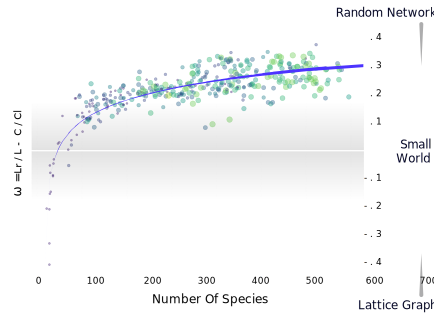
\includegraphics[width=\textwidth]{figures_c3/logpart.pdf}
        \caption{\textbf{A figure showing the small worldness for many Monte-Carlo selected MCM subsets}. The network structure of these is then assessed using the omega coefficient, with [-1,0,1] corresponding to the perfect lattice, small-world and random network structure. Here Node size and colour represents the number of reactions in the subset and the number of primary VOCs (blue=small, green=large).}
        \label{fig:smw}
\end{figure}



\subsection{Power Law and Scale-free graphs}
In real-world applications, it is common to have a hierarchical structure. These are often seen in the increase of citation counts in academic papers \citep{scalefreepapers}, email threads \citep{scalefreeemail} and the world wide web \citep{neoj4}. Unlike random or small-world graphs, scale-free graphs take a hub-and-spoke structure (\autoref{fig:gstructure}), which follows a power-law distribution - that is that scaling probability $p(x) \propto x^{-\alpha}$, where $\alpha$ is a constant and known as the scaling parameter.

\cite{scalefreebad} suggests that scale-free networks are rare, and often misdiagnosed with incorrect tests, or the misinterpretation of power-law features in a network. Similarly, \cite{plexp} suggests that even if the data distribution of a graph is well represented by the power-law distribution, in many cases a logarithmic or exponential distribution may have a better fit. 

\begin{figure}[H]
     \centering
         \includegraphics[width=.8\textwidth]{figures_c3/graphstyles.png}
        \caption{\textbf{The different network structures}. A visual depiction of the different graph structures. Source: \cite{neoj4}}
        \label{fig:gstructure}
\end{figure}

To assess the best distribution for describing the monte carlo subsets of the MCM I use the Kolomogorov-Smirnov statistic \citep{ks}. This calculates the maximum distance $D$ between the selected cumelative distribution function $S(x)$ (In our case the Logarithmic, Exponential and Power Law) of the data and the fitted model $P(x)$:

\begin{equation}
D = \smash{\displaystyle\max_{x \ge x_{min}}} |{S(x) - P(x)}|
\end{equation}

Using the MCM subsets from before \autoref{fig:ksd} shows that out of the three tested distributions, the MCM is best represented as a power-law distribution. Although this is not entirely within the chosen 5\% significance, it is highly indicative that some aspects of the network are scale-free.

\begin{figure}[H]
     \centering
         \includegraphics[width=\textwidth]{figures_c3/KSdistance.png}
        \caption{\textbf{Comparing the MCM subsets against a power law, logarithmic and exponential distribution.} The fit for different cumulative probability distributions of nodes in the MCM network is compared to determine the type of network hierarchy the chemistry follow. This is done by comparing the distance of the calculated distribution of data against a perfect one using the Kolomogorov-Smirnov test. The closer the two distributions are the better the fit. }
        \label{fig:ksd}
\end{figure}

\subsection{Describing the MCM network}
To conclude the MCM network exhibits both small world and scale-free (power-law) characteristics. This agrees with previous knowledge about the apparent network structure (branch and core - ref CH1/2). Here large primary emitted hydrocarbons produce branches of a hierarchical nature, as they are progressively broken down into smaller species. Since smaller species are then able to react with a much greater range of species, they then begin to form a tightly connected core, which exhibits many small-world features. This can be seen as the densely connected region within the graphs in CHAPTER !. 

Having classified the MCM network type, the next section will look at how MCM based simulation results can be converted into the graph structure for more in-depth analysis, \autoref{sec:metriccase}.
